\chapter{Sistem Analizi}

Projenin hedefi, eldeki sensör verilerinden çıkarımda bulunarak kullanıcının o anki ulaşım türünün tespit edilmesidir. Sensör verilerinin işlenmesi ve çıkarımda bulunulabilmesi için ise çıkarım mekanizmasına ihtiyaç duyulmaktadır. Bu mekanizmayı oluşturmak için makine öğrenmesi teknikleri kullanılmıştır. Makine Öğrenmesi (Machine Learning), matematiksel ve istatistiksel yöntemler kullanarak mevcut verilerden öğrenim modeli veya başka bir deyişle çıkarım mekanizması oluşturur. Bu model aracılığı ile bilinmeyene dair tahminlerde bulunur. 

Projede makine öğrenmesi tekniklerinin kullanılması bazı ihtiyaçları ortaya koymaktadır. Yukarıda belirtilen çıkarım mekanizmasının oluşturulabilmesi için her bir vasıta ile yapılmış yolculuklara ait ivmeölçer ve jiroskop sensör verilerine ihtiyaç duyulmaktadır. İhtiyaç duyulan bu veri seti Şekil 4.1'de genel yapısı gösterilen sistem aracılığı ile elde edilmiştir.

\begin{figure}[!htbp]
\centering
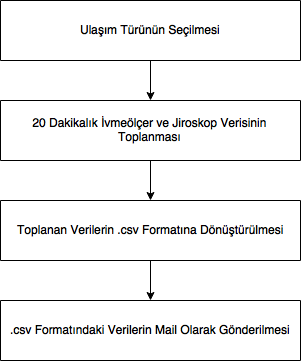
\includegraphics[scale=0.6]{projectChapters/images/genelakis.png}
\caption{Sensör veri seti oluşturmak için gerekli sistemin genel diyagramı}
\end{figure}

%Projede gözetimli öğrenme (supervised learning) tekniğinin kullanılacak olması makine öğrenmesi algoritmasına veri seti sunmamızı gerektirmektedir. Gözetimli öğrenme, algoritmaya sunulan veri setinden bir model çıkarıp daha sonrasında bilgisayarın bu model üzerinden yeni verileri sınıflandırması işlemidir. Bu nedenle projede makine öğrenmesi modeli oluşturmak için kullancıların her bir vasıta ile yaptığı seyahatler esnasında topladığı sensör verilerine ihtiyaç duyulmaktadr. Bu verileri toplamak için bir uygulama geliştirilmesi gerekmektedir. Bu uygulamaya ait kullanım senaryosu ve veri akış diyagramı aşağıdaki gibidir.
Tasarlanan sisteme ait kullanım senaryosu Şekil 4.2'de ve veri akış diyagramı Şekil 4.3'de görülmektedir.
\vspace{5mm}
\begin{figure}[!htbp]
\centering
\includegraphics[scale=0.6]{projectChapters/images/UseCase1.png}
\caption{Sensör veri toplama uygulamasına ait kullanım senaryosu}
\end{figure}

Kullanıcı veri toplayacağı araç tipini belirledikten sonra başlama komutunu verir ve jiroskop ile ivmeölçere ait veriler toplanmaya başlanır. Bu veriler 20 dakika toplandıktan sonra veritabanına kaydedilir. Veritabanında her bir sensörün 3 eksenine ait veriler ve verilerin toplandığı araç tipi bulunmaktadır.
Kullanıcı toplanan verileri listeleyebilmektedir. Yanlış veri toplanmış ise kullanıcı bu verileri silebilmektedir. Toplanan verilerin bilgisayar ortamına aktarılması gerekmektedir. Verilerin mail yoluyla gönderilmesi tercih edilmiştir. İlk olarak sensör verileri CSV formatına dönüştürülür. Daha sonrasında bu dosya alıcıya mail olarak gönderilir.

\begin{figure}[!htbp]
\centering
\includegraphics[scale=0.5]{projectChapters/images/VeriAkis1.png}
\caption{Sensor Veri Toplayıcısına ait veri akış diyagramı}
\end{figure}

Sensör verilerinden oluşan ham veri setinin makine öğrenmesi algoritmalarına girdi olarak verilebilmesi için hazır olması gerekmektedir. Ham veri setine ait veriler ilk olarak özellik çıkarımı işleminden geçirilir. Veri setinden çıkarılacak özellikler daha önceden eğitim verisi üzerinde belirlenmektedir. Özellik çıkarımı işlemi ile beraber oluşturulan yeni veri seti makine öğrenmesi modelinden geçirilecek hale gelmiş olur. Uygulama içerisinde kullanılacak olan modelin belirlenmesi işlemi Weka üzerinde daha önceden yapılır. Toplanan eğitim verileri özellik çıkarımı ve özellik seçimi işleminden geirildikten sonra elde edilen yeni veri seti makine öğrenmesi algoritmalarından geçirilir. En yüksek doğruluk değerini veren algoritmanın oluşturduğu makine öğrenmesi modeli uygulama içerisinde kullanılır.

Kullanıcının ulaşım türünün tespit eden sistemin genel akış diyagramı Şekil 4.5'de görülmektedir.

\begin{figure}[!htbp]
\centering
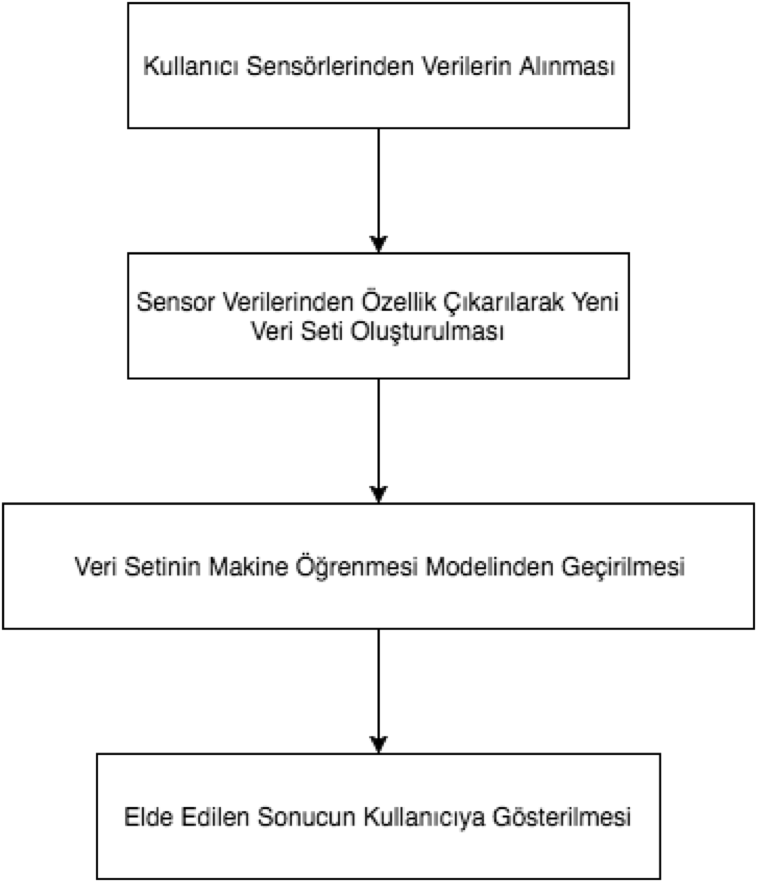
\includegraphics[scale=0.8]{projectChapters/images/yazilimTasarimi.png}
\caption{Sistem yapısına ait blok diyagram}
\end{figure}
\newpage
\begin{figure}[!htbp]
\centering
\includegraphics[scale=0.6]{projectChapters/images/UseCase2.png}
\caption{Ulaşım türünü tespit eden uygulamaya ait kullanım senaryosu}
\end{figure}

Veri seti makine öğrenmesi modelinden geçirildikten sonra elde edilen sonuç kullanıcıya gösterilir. Sonuç bilgisi, kullanıcının anlık ulaşım türünün hangi vasıta olduğunu içerir. Bu bilgi daha sonrasında veritabanına kaydedilir. Bu sayede kullanıcı ulaşım türü geçmişine bakabilmektedir. Aşağıda kullanıcının anlık ulaşım türünün tespit edilmesini sağlayan uygulamanın kullanım senaryosu ve veri akış diyagramı bulunmaktadır.

\begin{figure}[!htbp]
\centering
\includegraphics[scale=0.5]{projectChapters/images/VeriAkis2.png}
\caption{Ulaşım türünü tespit eden uygulamaya ait veri akış diyagramı}
\end{figure}